\section*{Paradigme numérique}
\addcontentsline{toc}{section}{Paradigme numérique}

En général, on suppose $\eps \ll 1$, et donc le système~\eqref{sec:intro:eq:u} comporte une dynamique \textit{rapide} par rapport au temps d'étude. À cet égard, des méthodes d'\textit{analyse asymptotique} ont été développées, c'est-à-dire des méthodes qui permettent de caractériser le système dans cette limite $\eps$ \enquote{petit}, en général en découplant ces deux dynamiques. Pour les problèmes hautement-oscillants, trois exemples particulièrement célèbres sont les méthodes d'homogénéisation~\cite{goudon.2003.homogenization}, de moyennisation~\cite{perko.1969.higher,sanders.2007.averaging,lochak.1988.multiphase} et de formes normales~\cite{murdock.2006.normal,bambusi.2003.birkhoff}. Pour les problèmes à relaxation rapide, la littérature est moins fournie. Qu'il s'agisse de calculer la variété centrale comme précédemment ou d'un développement de Chapman-Enskog~\cite{santos.1986.divergence,degond.2004.macroscopic,chartier.2015.uniformly}, la phase transitoire n'est pas calculée. 

Plus récemment dans \cite{castella.2016.formal}, les auteurs capturent aussi la phase transitoire, mais la méthode est très difficile à s'approprier et n'est valide que dans la limite $\eps \rightarrow 0$. Dans cette section, on étudie l'application de méthodes numériques \enquote{standards} de l'état de l'art, et on observe le comportement de l'erreur numérique non seulement en fonction du pas de temps $\Dt$, mais aussi en fonction du paramètre $\eps$. 

Dans cette section, on commence par décrire ce qu'on entend par \enquote{méthode numérique} et le contexte dans lequel on va les étudier. Ensuite, on présente trois méthodes d'ordre 2 reconnues dans l'état de l'art~: le splitting de Strang, un schéma IMEX-BDF et une méthode de Runge-Kutta exponentielle. 



\subsection*{Mise en place de la résolution}
\addcontentsline{toc}{subsection}{Mise en place de la résolution}

Pour étudier le comportement des schémas numériques sur les problèmes de la forme~\eqref{sec:intro:eq:u}, on considère l'exemple jouet suivant
\begin{subequations} \label{sec:intro:eq:jouet_v}
    \begin{empheq}[left=\left\lbrace, right=\right.]{align} &
        \pa_t v_1 = v_2 , & &
        v_1(0) = 1 , \vphantom{\frac11}\qquad\qquad
        \\ & 
        \pa_t v_2 = -\frac{1}{\eps}\big( v_1 + v_2 \big) , & &
        v_2(0) = 0 .
    \end{empheq}
\end{subequations}
Cet exemple ressemble à certains problèmes hyperboliques avec relaxation, et sa linéarité le rend simple à étudier. Il prend facilement la forme~\eqref{sec:intro:eq:xz} en posant par exemple $x = v_1$ et $z = v_1 + v_2 $, ce qui donne 
\begin{subequations} \label{sec:intro:eq:jouet_xz}
    \begin{empheq}[left=\left\lbrace, right=\right.]{align} &
        \pa_t x = -x + z , & &
        x(0) = 1 , \vphantom{\frac11}\qquad\qquad
        \\ & 
        \pa_t z = -\frac{1}{\eps}z - x + z , & &
        z(0) = 1 .
    \end{empheq}
\end{subequations}
Ce problème est linéaire et se diagonalise sans problème pour $\eps < 1/4$, ce qui génère
\begin{equation*}
    \newcommand{\sqEps}{\sqrt{1 - 4\eps}}
    \tilde{u} = \underbrace{\begin{pmatrix}
        -1 & 1 - r_\eps \\
        \eps & 1 - \eps - \eps r_\eps 
    \end{pmatrix}}_{\displaystyle P} \begin{pmatrix} x \\ z \end{pmatrix},
    \qquad\text{tel que}\qquad
    \pa_t \tilde{u} = \begin{pmatrix}
        -r_\eps & 0 \\ 0 & -\frac{1}{\eps} + r_\eps
    \end{pmatrix} \tilde{u}
\end{equation*}
avec $r_\eps = \frac{1}{2\eps} \big( 1 - \sqrt{1 - 4\eps} \big)$. On obtient directement une expression explicite pour $u = \among{x}{z}$, qui est 
\begin{equation*}
    u(t) = P^{-1} \begin{pmatrix}
        e^{-t r_\eps} & 0 \\ 0 & e^{-t/\eps} e^{t r_\eps}
    \end{pmatrix} P u(0) 
\end{equation*}
où $P^{-1} = \frac{1}{\sqrt{1 - 4\eps}} \begin{pmatrix}
    -1 + \eps + \eps r_\eps  &  1 - r_\eps \\
                \eps         &      1
\end{pmatrix}$.
\begin{FRremark*}
    On voit bien dans la définition de $r_\eps$ que le problème change de nature entre $\eps \leq 1/4$ et $\eps > 1/4$. En effet, dans le premier cas le système est purement dissipatif, alors que dans le second, des oscillations apparaissent. Cette singularité apparaît également dans la matrice de changement de variable, dont le déterminant vaut $-\sqrt{1 - 4\eps}$.
\end{FRremark*}


\paragraph{Introduction aux résolutions numériques\\}
Dans les faits, on ne saura pas résoudre tous les systèmes de la forme~\eqref{sec:intro:eq:u} de manière exacte. Donc on va appliquer des méthodes d'\textit{approximation numérique} pour calculer une solution approchée. À partir l'exemple~\eqref{sec:intro:eq:jouet_xz}, on va étudier la précision de ces méthodes.

\todo[inline]{Discrétisation de $t$ de manière uniforme}

\todo[inline]{\textbf{Def :} erreur d’une méthode numérique, notion d'erreur uniforme en $\eps$}

\todo[inline]{\textbf{Rq :} on pourrait considérer une interpolation des données et définir une erreur dans le monde continu mais c’est compliqué et déjà si l'erreur ponctuelle est bien on est content}

\todo[inline]{\textbf{Rq:} De par sa structure, on sait calculer $\exp(-t A)$ pour Strang ou expRK, ou qu’on sait facilement inverser $\id + \Dt \, A$ pour IMEX-BDF.}

\todo[inline]{\textbf{Def :} ce qu’on entend par un schéma numérique, 
\vspace*{-12pt}
$$u_{n+s} = u_{n+s-1} + \Dt\, \Phi^{\eps}_{\Dt} (u_{n+s-1}, \ldots, u_n)$$
\vspace*{-24pt}}

\todo[inline]{Footnote : en vérité, quitte à remplacer $u_n$ par $U_n = (u_{n+s-1}, \ldots, u_n)$, on peut se ramener à des méthodes à une seule étape}


\subsection*{Méthodes numériques}
\addcontentsline{toc}{subsection}{Méthodes numériques}

On présente les résultats associés à trois méthodes d'ordre 2, qui traitent la partie raide différemment de la partie non-raide. Les méthodes sont bien définies  dans la limite $\eps \rightarrow 0$, et on le comportement de l’erreur en fonction de $\Dt$ \textit{et} de $\eps$.

On ne considère pas de méthodes complètement implicites parce qu'elles sont très coûteuses et pas très adapté pour l'extension aux EDP... Néanmoins la convergence des méthodes implicites est souvent excellente et des implémentations très efficaces existent. La référence sur le sujet est~\cite{hairer.1996.solving}, et toutes les bonnes boîtes à outils de résolution d'EDO contiennent la méthode RadauII.\footnote{Attention cependant, la plupart de ces boîtes à outils masquent la difficulté associée aux méthodes implicites, qui sont la résolution d'un système et de l'erreur associée. En outre, il est parfois difficile de désactiver le pas de temps adaptatif, ce qui est problématique pour une étude de convergence.} On ne considère pas non plus de méthodes purement explicites demandent $\Dt < \eps$, ce qui est beaucoup trop coûteux. 

Il est important de noter que ce manuscrit ne présente pas une étude des schémas présentés. Il s'agit simplement d'une compilation non-exhaustive de résultats et d'observations rapides sur les propriétés de ces méthodes appliquées à~\eqref{sec:intro:eq:u} afin de contextualiser les contributions du manuscrit par la suite.



\paragraph{Splitting de Strang\\}

Une approche courante est de séparer le problème~\eqref{sec:intro:eq:u} en deux parties, une raide et une non-raide. La manière naturelle de procéder fournit
%
\begin{empheq}[left=\left\lbrace, right=\right.]{align*} &
    \pa_t u^{(1)} = -\frac{1}{\eps}A u^{(1)} ,
    \\ &
    \pa_t u^{(2)} = f(u^{(2)}) . \vphantom{\frac11}
\end{empheq}
%
On note $\varphi_t$, $\varphi^{(1)}_t$ et $\varphi^{(2)}_t$ les $t$-flots associés aux problèmes en $u$, $u^{(1)}$ et $u^{(2)}$ espectivement. On remarque qu'il est simple de calculer $\varphi^{(1)}$ de manière exacte, et simple de calculer $\varphi^{(2)}$ de manière numérique. Cependant, ces deux dynamiques sont mélangées dans $\varphi$, ce qui rend le flot du problème d'origine difficile à calculer. Ainsi, on est en droit de se poser la question~: Est-il possible d'obtenir $\varphi$ à partir de $\varphi^{(1)}$ et de $\varphi^{(2)}$~? 

La réponse est non en général, mais on peut \textit{approcher} $\varphi$ à partir des autres avec des compositions successives. C'est cette approche qu'on appelle \textit{splitting}. Le plus couramment utilisé est le splitting de Strang, qui s'écrit 
\begin{equation*}
    \varphi_t = \varphi^{(1)}_{t/2} \circ \varphi^{(2)}_{t} \circ \varphi^{(1)}_{t/2} + \bigO(t^3) .
\end{equation*}
Pour la plupart des équations, l'ordre des opérations n'a pas d'importance, mais lorsque le système présente une partie de relaxation raide comme ici, il a été remarqué dans~\cite{sportisse.2000.analysis,descombes.2004.operator} qu'il vaut mieux \enquote{terminer} par la relaxation. 

Notons que le splitting de Strang peut être obtenu par symétrie à partir du splitting de Lie $\Phi_t = \varphi^{(2)}_{t} \circ \varphi^{(1)}_{t}$, d'ordre 1. 
% Attention, $\Phi_t$ n'est pas un $t$-flot au même sens que $\varphi_t$, c'est la solution particulière d'une EDO dans l'espace des morphismes. Dans le cas où $f$ est linéaire, on dispose de la formule de Baker-Campbell-Hausdorff (BCH),\todo{REF BCH}
% \begin{equation*}
%     \log \big( \Phi_t \big)
%     = t\left(\frac{-1}{\eps}A + f\right) 
%     - \frac{t^2}{2\eps} \left[A, f\right]
%     + \frac{t^3}{12\eps^2}\big( [A,[A,f]] + \eps [f,[A,f]] \big)
%     + \ldots
% \end{equation*}
% avec $[f,g] = fg - gf$ le commutateur de champs linéaires. Cette formule n'est valide que formellement, c'est-à-dire qu'elle ne converge pas forcément et que l'important est le terme général qui la génère. On peut la comparer à un développement de Taylor qu'on a poussé à un ordre \enquote{infini}. L'objet obtenu est une série entière en $t$, mais celle-ci peut avoir un rayon de convergence nul. Néanmoins, les termes de la série ont du sens et on peut en prendre les premiers termes pour construire des approximations, bien qu'il faille être prudent avec la régularité de la fonction pour obtenir des résultats rigoureux.
Le splitting est exact si et seulement si les champs $A$ et $f$ commutent, c'est-à-dire si on vérifie l'identité 
\begin{equation*}
    Af - \pa_u f \cdot A = [A,f] = 0 .
\end{equation*}
Dans ce cas, le splitting de Lie génère un flot qui coïncide avec $\varphi$. Évidemment, ce n'est pas le cas en général. En particulier dans le cas test~\eqref{sec:intro:eq:jouet_xz}, on a $[A,f] = \begin{pmatrix} 0 & -1 \\ -1 & 0 \end{pmatrix}$, donc on s'attend à avoir une erreur qui décroit comme $\Dt^2$ lors de la simulation. Cependant, on observe un résultat différent en Figure~\ref{sec:intro:fig:strang}.


% \begin{itemize}
%     \item Le morphisme $\Phi_t$ est un flot;
%     \item $\Phi_t$ et $\varphi_t$ coincïdent en tout $t$;
%     \item Les champs $A$ et $f$ commutent.
% \end{itemize}
% Le morphisme $\Phi_t$ est un flot si et seulement si cette expression est linéaire en $t$, or ce n'est pas le cas en général. Le seul moyen que ce soit le cas est que $A$ et $f$ commutent. Ce résultat est aussi valide dans le cas non-linéaire, avec le commutateur
% \begin{equation*}
%     [f,g] = \pa_u f \cdot g - \pa_u g \cdot f 
% \end{equation*}
% qui définit une algèbre de Lie sur les champs de vecteurs. Ceci correspond à une manière plus géométrique de considérer les champs de vecteurs qui revient à les associer à l'opérateur de transport $\mathcal{D}_f(g) = \pa_u g \cdot f$. Ainsi, $[f,g] = \mathcal{D}_g(f) - \mathcal{D}_f(g)$. 

% On définit l'erreur de splitting 
% \begin{equation*}
%     \err_{\mathrm{Lie}} 
%     = \log \big( \Phi_t \big) - t\left(\frac{-1}{\eps}A + f\right) 
% \end{equation*}
% qui permet d'obtenir l'erreur de troncature du schéma par un passage à l'exponentielle. Il apparaît à partir de la formule de BCH que cette erreur est de taille $t^2/\eps$, pas indépendante de $\eps$. Néanmoins, on a déjà vu avec Euler implicite que l'accumulation d'erreur pouvait devenir indépendante de $\eps$, grâce aux propriétés de décroissance de $z$. C'est le cas ici, et on peut borner l'erreur \textit{indépendamment} de $\eps$. 

% On cherche ensuite à améliorer la convergence du schéma: il serait agréable de pouvoir profiter d'une convergence à un ordre plus élevé. La méthode généralement considérée est le splitting de Strang~:
% \begin{equation*}
%     \varphi_t \approx \varphi^{(1)}_{t/2} \circ \varphi^{(2)}_{t} \circ \varphi^{(1)}_{t/2} .
% \end{equation*}
% Cette méthode a l'avantage d'être d'ordre 2, et de présenter des propriétés géométriques sympathiques de par sa symétrie (elle génère d'ailleurs la méthode de Störmer-Verlett, voir Annexe~\textbf{REF}\todo{Storm-Verl}). Néanmoins, il n'est pas clair qu'elle présente un bon comportement lorsque la raideur augmente, i.e. lorsque $\eps$ diminue. En effet, un calcul de l'erreur de troncature donne 
% \begin{equation*}
%     \varphi_t - \varphi^{(1)}_{t/2} \circ \varphi^{(2)}_{t} \circ \varphi^{(1)}_{t/2} 
%     = \frac{t^3}{12\eps^2} \big( [A,[A,f]] + \eps [[A,f],f] \big)
%     + \bigO(t^4) .
% \end{equation*}
% Ainsi, même si un $1/\eps$ est compensé par la décroissance rapide de $z$, l'erreur ne sera pas indépendante de $\eps$. On peut vérifier ce résultat de manière numérique.


\begin{figure}
    \centering
    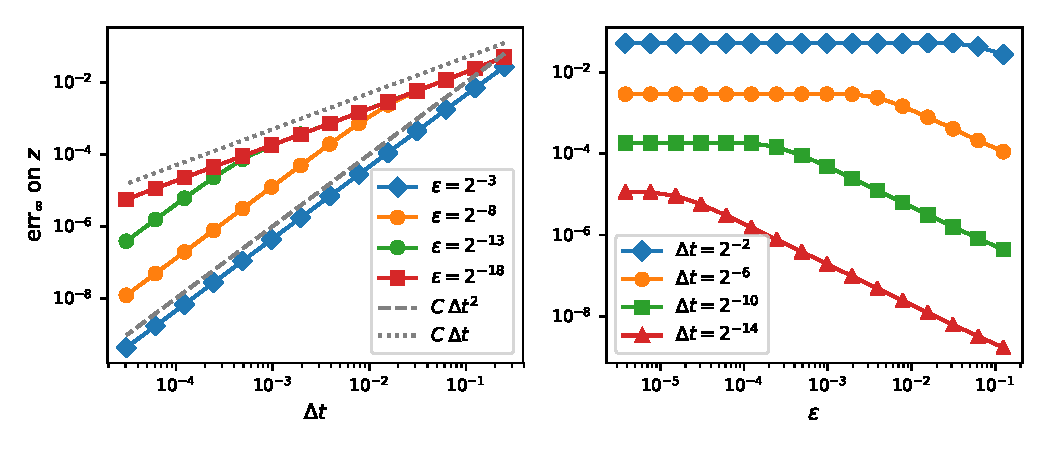
\includegraphics[width=\textwidth]{./Presentation/strang_err_x.pdf}
    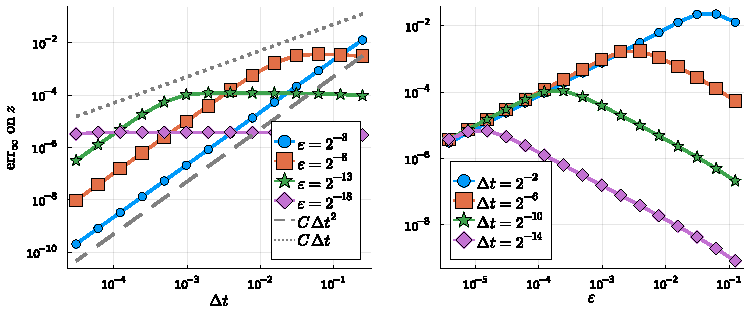
\includegraphics[width=\textwidth]{./Presentation/strang_err_z.pdf}
    \caption{Erreurs sur $x$ (en haut) et $z$ (en bas) en fonction de $\Dt$ (à gauche) et de $\eps$ (à droite) avec la méthode de Strang. Sur les tracés de l'erreur en fonction de $\Dt$, les convergences théorique et uniforme sont tracées.}
    \label{sec:intro:fig:strang}
\end{figure}

Dans cette figure, on observe que le comportement de la solution est le bon attendu pour $\Dt \ll \eps$. Néanmoins, lorsqu'on trace l'erreur en fonction de $\eps$, on voit qu'à $\Dt$ fixé, il y a toujours un seuil à partir duquel une réduction de $\eps$ entraîne une augmentation de l'erreur. Cette augmentation entraîne une \textit{réduction d'ordre}, c'est-à-dire qu'on ne peut pas avoir
\begin{equation*}
    \sup_{0 < \eps \leq \eps_0} \err \leq C \Dt^q ,
\end{equation*}
avec $q = 2$, ce n'est possible qu'avec $q = 1$. Cette réduction d'ordre a été notée dans différents contextes \cite{sportisse.2000.analysis,faou.2015.analysis}, et différentes méthodes ont été développées pour dépasser cette limite \cite{einkemmer.2015.overcoming,cano.2017.avoiding,bertoli.2020.strang}, en particulier l'utilisation de schémas dits \enquote{exponentiels}. 

\todo[inline]{Expliquer un peu mieux les graphes}
\todo[inline]{Faire une colormap d'erreur avec $\Dt$ et $\eps$ en coordonnées pour mieux discuter du comportement asymptotique $\eps \rightarrow 0$ du schéma.}


\paragraph{Méthodes exponentielles Runge-Kutta (expRK)\\}

Ces méthodes exponentielles\footnote{À ne pas confondre avec les méthodes de Lawson (voir~\cite{lawson.1967.generalized,hochbruck.2020.convergence}) qui procèdent en applicant des méthodes de Runge-Kutta standards sur la variable filtrée $v(t) = e^{t A/\eps}u(t)$, puis en multipliant le résultat par $e^{-t A/\eps}$. Les résultats théoriques sur la convergence de ces dernières sont encore très récents.} proviennent de la formulation intégrale
\begin{equation*}
    u(t) = e^{-\frac{t}{\eps}A}u_0 + \int_0^t e^{-\frac{t-\tau}{\eps}A} f(u(s)) \D s .
\end{equation*}
La partie du semi-groupe est gardée exacte tandis que la partie (possiblement) non-linéaire est approchée, ce qui engendre à l'ordre 1 le schéma
\begin{equation} \label{sec:intro:eq:expEuler}
    u_{n+1} = e^{-\Dt A/\eps} u_n + \left(\int_0^{\Dt} e^{(\tau-\Dt) A/\eps} \D\tau \right) f(u_n) .
\end{equation}
Pour passer à l'ordre supérieur, les parties raide et non-raide sont liées, donc l'approche demande plus de subtilité, mais on peut obtenir des méthodes exponentielles Runge-Kutta (i.e. des méthodes à un pas, pour obtenir $u_{n+1} \approx u(t_{n+1})$ à partir de seulement $u_n \approx u(t_n)$) d'ordre arbitraire. Une grande classe de schémas de ce type est compilée dans~\cite{hochbruck.2005.explicit}, et dans un autre article les mêmes auteurs obtiennent une convergence théorique. 
\begin{FRtheorem*}[Hochbruck, Ostermann - \cite{hochbruck.2004.exponential}]
    Avec un schéma expRK d'ordre~$q \geq 1$, l'erreur vérifie la borne à une constante multiplicative près
    \begin{equation*}
        \left| 
            \left( I + \frac{1}{\eps}A \right) \big( u_n - u(t_n) \big) 
        \right|
        \leq \Dt^{q} \left( 
            \sup_{0 \leq t \leq t_n} \big| \pa_t^{\: q-1} \mathcal{U}(t) \big| 
            + \int_0^{t_n} \big| \pa_t^{\: q} \mathcal{U}(t) \big| \D t 
        \right) 
    \end{equation*}
    où $\mathcal{U} = \pa_t u + \frac{1}{\eps}Au$. 
\end{FRtheorem*}
\noindent%
Ce théorème est en général évoqué dans un contexte fonctionnel de problème parabolique, mais cette version simplifiée est suffisante ici. Un intérêt remarquble de ces méthodes est que dans l'erreur, la composante~$z$ est renormalisée par~$\eps$. Dans notre cas, cela permet d'obtenir une sorte d'erreur relative puisque $z(t) = \eps h^\eps(x(t)) + \bigO(e^{-t/\eps})$. D'ailleurs, le schéma~\eqref{sec:intro:eq:expEuler} (parfois appelé \enquote{Euler exponentiel}) avait été proposé dans~\cite{verwer.1998.note} pour obtenir une meilleur convergence que le splitting de Strang en erreur relative. 

\begin{figure}
    \centering
    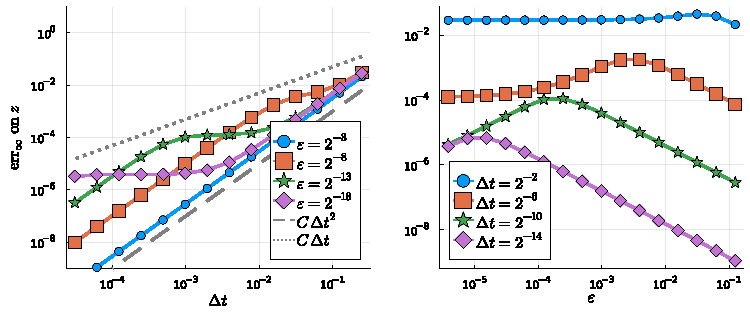
\includegraphics[width=\textwidth]{./Presentation/rk2_err_x.pdf}
    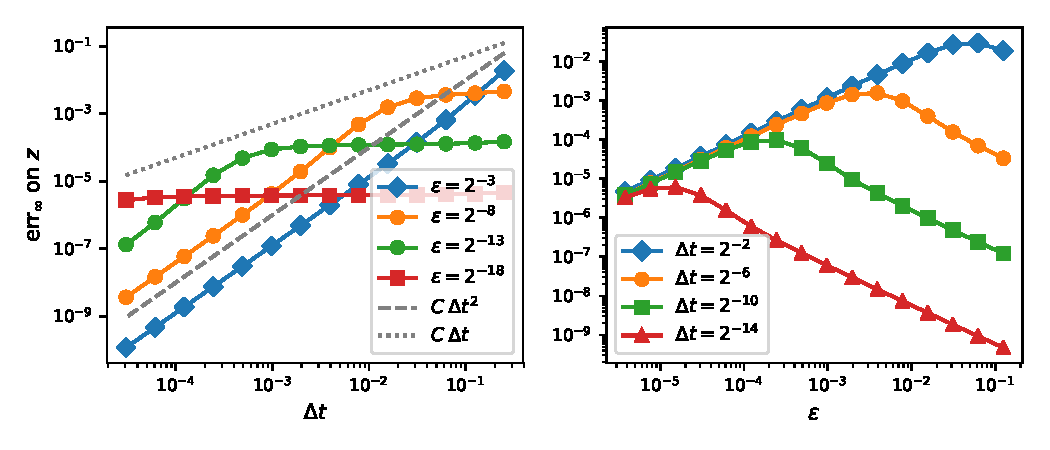
\includegraphics[width=\textwidth]{./Presentation/rk2_err_z.pdf}
    \caption{Erreurs sur $x$ (en haut) et $z$ (en bas) en fonction de $\Dt$ (à gauche) et de $\eps$ (à droite) avec le schéma exponentiel RK2. Sur les tracés de l'erreur en fonction de $\Dt$, les convergences théorique et uniforme sont tracées.}
    \label{sec:intro:fig:rk2}
\end{figure}

Cette renormalisation par~$\eps$ de la composante~$z$ se voit nettement en Figure~\ref{sec:intro:fig:rk2}. On remarque aussi qu'à $\eps$ fixé, l'erreur sur~$x$ en fonction de $\Dt$ semble présenter trois phases:
\begin{itemize}
    \item une décroissance en $Dt^2$;
    \item un plateau à partir de $Dt^2 \approx \eps$ jusqu'à $\Dt \approx \eps$;
    \item de nouveau une décroissance en $\Dt^2$.
\end{itemize}
Cette seconde phase engendre une réduction d'ordre, où l'ordre \enquote{uniforme} est 1. Pour la composante~$z$, il n'y a pas de première phase, mais la réduction d'ordre est la même. Malgré cela, la convergence est meilleure que pour le splitting de Strang~: si on reste dans le paradigme $\Dt^2 > \eps$ avec $\eps \rightarrow 0$, l'erreur sur~$x$ décroit comme $\Dt^2$ et l'erreur sur $z$ est presque nulle. Cette notion de convergence en $\Dt^2$ sans pouvoir passer à la limite $\Dt \rightarrow 0$ va à l'encontre des notions usuelles de convergence, et bien que ces précautions soient rarement prises dans la littérature. On dit que le schéma \enquote{préserve l'asymptote}.

\todo[inline]{Faire une colormap d'erreur avec $\Dt$ et $\eps$ en coordonnées pour mieux discuter du comportement asymptotique $\eps \rightarrow 0$ du schéma. Notamment, si on pose $\eps = 0$ la convergence est d'ordre 2.}



\paragraph{Méthode IMEX-BDF\\}


Le souci des méthodes exponentielles est qu'elles demandent une intégration très précise du semi-groupe $t \mapsto e^{-tA/\eps}$. On peut considérer des méthodes moins coûteuses, qui demandent seulement d'inverser un système linéaire. À cet égard, on peut considérer des méthodes implicite-explicites (IMEX), où la partie raide est implicite et la partie non-linéaire est explicite. Par exemple la méthode d'Euler implicite-explicite appliquée à~\eqref{sec:intro:eq:u} donne
\begin{equation*}
    \frac{u_{n+1} - u_n}{\Dt} = -\frac{1}{\eps}A u_{n+1} + f(u_n) .
\end{equation*}
On se restreint ici aux méthodes multipas dénommées IMEX-BDF (\textit{backwards differentiation formula}), initialement développées dans~\cite{crouzeix.1980.methode}, puis dans~\cite{ascher.1995.implicit,akrivis.1999.implicit,hundsdorfer.2007.imex,dimarco.2017.implicit}. On a là aussi une erreur théorique.

\begin{FRtheorem*}[Crouzeix - \cite{crouzeix.1980.methode}]
    On peut borner l'erreur d'une méthode IMEX-BDF d'ordre~$q$ à~$s$ pas par
    \begin{equation*}
        \big| u_n - u(t_n) \big| \leq
        \sum_{i = 0}^{s-1} \big| u_i - u(t_i) \big|
        + \Dt^q \int_0^{t_n} \left( 
            \big| \pa_t^{\: q+1} u(t) \big| 
            + \frac{1}{\eps} \big| A \pa_t^{\: q} u(t) \big| 
        \right) \D t 
    \end{equation*}
    à une constante multiplicative près.
\end{FRtheorem*}

La différence principale de cette erreur avec celle des méthodes expRK est que la composante~$z$ n'est pas \enquote{normalisée}. On voit ainsi en Figure~\ref{sec:intro:fig:bdf2} que l'erreur uniforme sur $z$ dégénère à l'ordre \textit{zéro}. Il est même possible d'augmenter l'erreur en diminuant le pas de temps~$\Dt$. 

\begin{figure}
    \centering
    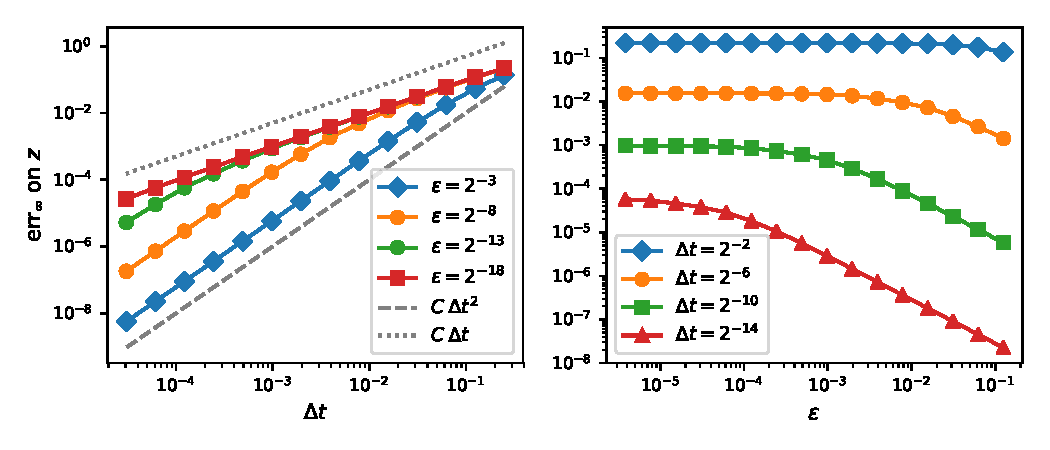
\includegraphics[width=\textwidth]{./Presentation/bdf2_err_x.pdf}
    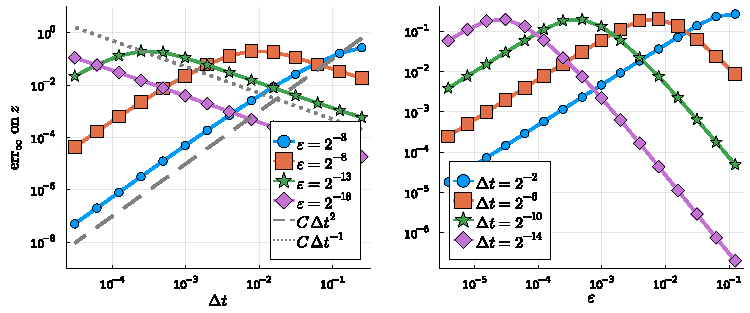
\includegraphics[width=\textwidth]{./Presentation/bdf2_err_z.pdf}
    \caption{Erreurs sur $x$ (en haut) et $z$ (en bas) en fonction de $\Dt$ (à gauche) et de $\eps$ (à droite) avec le schéma IMEX-BDF2. Sur les tracés de l'erreur en fonction de $\Dt$, les convergences théorique et uniforme sont tracées.}
    \label{sec:intro:fig:bdf2}
\end{figure}

Ces méthodes sont néanmoins très utilisées, notamment dans le contexte de modèles cinétiques. Par exemple les méthodes IMEX-LM développées dans~\cite{lemou.2008.new,boscarino.2017.unified,albi.2020.implicit} sur un système 
\begin{equation*}
    \pa_t \rho + \pa_x j = 0, \qquad 
    \pa_t j + \frac{1}{\eps} \pa_x \rho = -\frac{1}{\eps}j 
\end{equation*}
prennent implicite la partie en~$j$ en gardant explicite la partie en~$\rho$. Cela permet d'avoir des schémas qui se comporte bien dans la limite $\eps \rightarrow 0$ malgré la raideur sur le transport en~$\rho$. 

En outre, si la donnée initiale se situe proche de l'équilibre $z = \eps h^\eps(x)$ de sorte que $\pa_t^{\: q+1} u$ reste bornée dans la limite~$\eps \rightarrow 0$, alors on peut obtenir une convergence uniforme. On peut voir une interprétation de ce résultat en Figure~\ref{sec:intro:fig:bdf2_z0} où l'erreur sur~$z$ est améliorée en prenant une donnée initiale nulle.\footnote{Le même phénomène est observé pour le schéma expRK.} Ainsi, il est fréquent de choisir une donnée initiale bien posée et d'annoncer que ce type de schéma est \enquote{uniformément précis}, par exemple dans~\cite{jin.2000.uniformly,hu.2021.uniform}. La même confusion est faite pour les schémas IMEX-RK dans~\cite{boscarino.2009.class,boscarino.2017.unified}, par exemple. Néanmoins, le caractère uniforme de ces derniers est remis en question dans~\cite{hu.2021.uniform}.

\begin{figure}
    \centering
    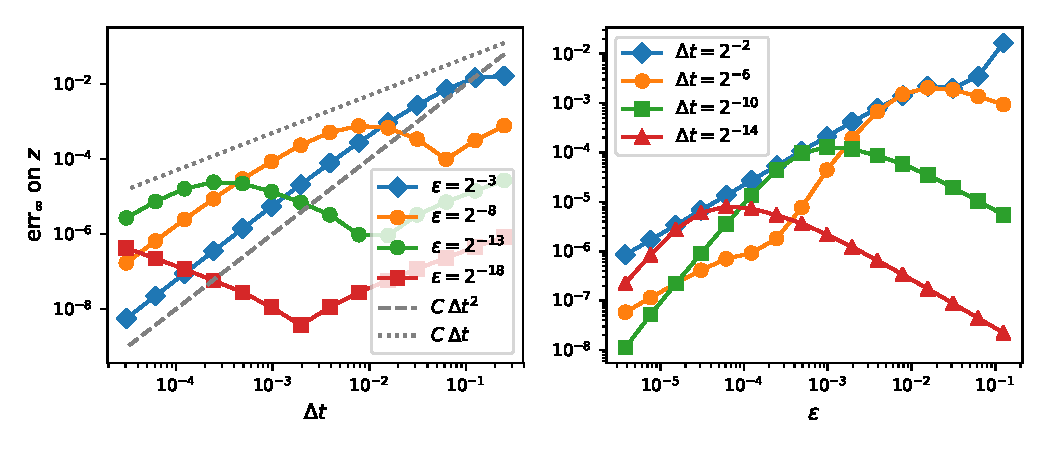
\includegraphics[width=\textwidth]{./Presentation/bdf2_err_z0.pdf}
    \caption{Erreur sur $z$ en fonction de $\Dt$ (à gauche) et de $\eps$ (à droite) avec le schéma IMEX-BDF2, avec une donnée initiale~$z(0) = 0$. Sur les tracés de l'erreur en fonction de $\Dt$, les convergences théorique et uniforme sont tracées.}
    \label{sec:intro:fig:bdf2_z0}
\end{figure}



\subsection*{Outils d'analyse des résultats}
\addcontentsline{toc}{subsection}{Outils d'analyse des résultats}

On voit que toutes ces méthodes subissent une réduction d'ordre: on passe d'une convergence à l'ordre~2 à une convergence d'ordre~1, ou pire. Pourtant, les schémas sont bien \textit{d'ordre~2}, comme on l'observe pour $\eps = 2^{-3}$. On voit bien l'intérêt d'introduire des concepts de convergence qui diffèrent des définitions usuelles. 

\begin{FRdefinition*}
    On distingue trois propriétés de convergence différentes pour les méthodes numériques~:
\begin{itemize}
    \item On dit qu'une méthode est \textit{asymptotic preserving} (AP) si, à condition initiale fixée indépendante de $\eps$, il est bien défini dans la limite $\eps \rightarrow 0$ et que son ordre n'est pas impacté par ce passage à la limite.
    \item On dit qu'une méthode est \textit{uniformly accurate} (UA) si, à condition initiale fixée indépendante de $\eps$, l'erreur uniforme (i.e. le supremum par rapport à $\eps$) a le même ordre que l'erreur du schéma.
    \item On dit qu'une méthode est \textit{UA à l'équilibre} si, pour une donnée initiale bien préparée, l'erreur uniforme (i.e. le supremum par rapport à $\eps$) a le même ordre que l'erreur du schéma.
\end{itemize}
\end{FRdefinition*}

\todo[inline]{Schéma de \enquote{commutation} avec $\rightarrow$ qui correspond à la discrétisation et $\downarrow$ à la limite en $\eps \rightarrow 0$. Être AP signifie commuter, être UA signifie pouvoir commuter même en faisant des \enquote{pauses} sur la flèches $\downarrow$.}

Toutes les méthodes présentées précédemment sont AP. Le splitting de Strang et le schéma IMEX-BDF2 donnent l'impression qu'avec $\eps \ll \Dt$, l'\enquote{ordre} dégénère à~1, mais en vérité c'est que l'écart entre $\eps$ et $\Dt$ n'est pas suffisant. Par contre il est clair qu'aucun n'est UA, bien que les méthodes IMEX-BDF et expRK sont UA à l'équilibre.
